\documentclass[10pt,twocolumn,letterpaper]{article}

\usepackage{cvpr}
\usepackage{times}
\usepackage{epsfig}
\usepackage{graphicx}
\usepackage{amsmath}
\usepackage{amssymb}

% Include other packages here, before hyperref.

% If you comment hyperref and then uncomment it, you should delete
% egpaper.aux before re-running latex.  (Or just hit 'q' on the first latex
% run, let it finish, and you should be clear).
\usepackage[pagebackref=true,breaklinks=true,letterpaper=true,colorlinks,bookmarks=false]{hyperref}

%%%%%%%%% PAPER ID  - PLEASE UPDATE
\def\cvprPaperID{0947} % *** Enter the CVPR Paper ID here
\def\httilde{\mbox{\tt\raisebox{-.5ex}{\symbol{126}}}}

\begin{document}

%%%%%%%%% TITLE - PLEASE UPDATE
\title{Guided Proofreading of Automatic Segmentations for Connectomics}  % **** Enter the paper title here

\maketitle
\thispagestyle{empty}

Thank you for your constructive comments. We will fix all minor issues.

\section{Quantitative Evaluation}



\section{Reproducibility}



\section{Optimal Parameters}



\section{Training Data Sets}



\section{Faster Correction Times}



\section{Merge Error Detection}

\begin{figure}[h]
\centering
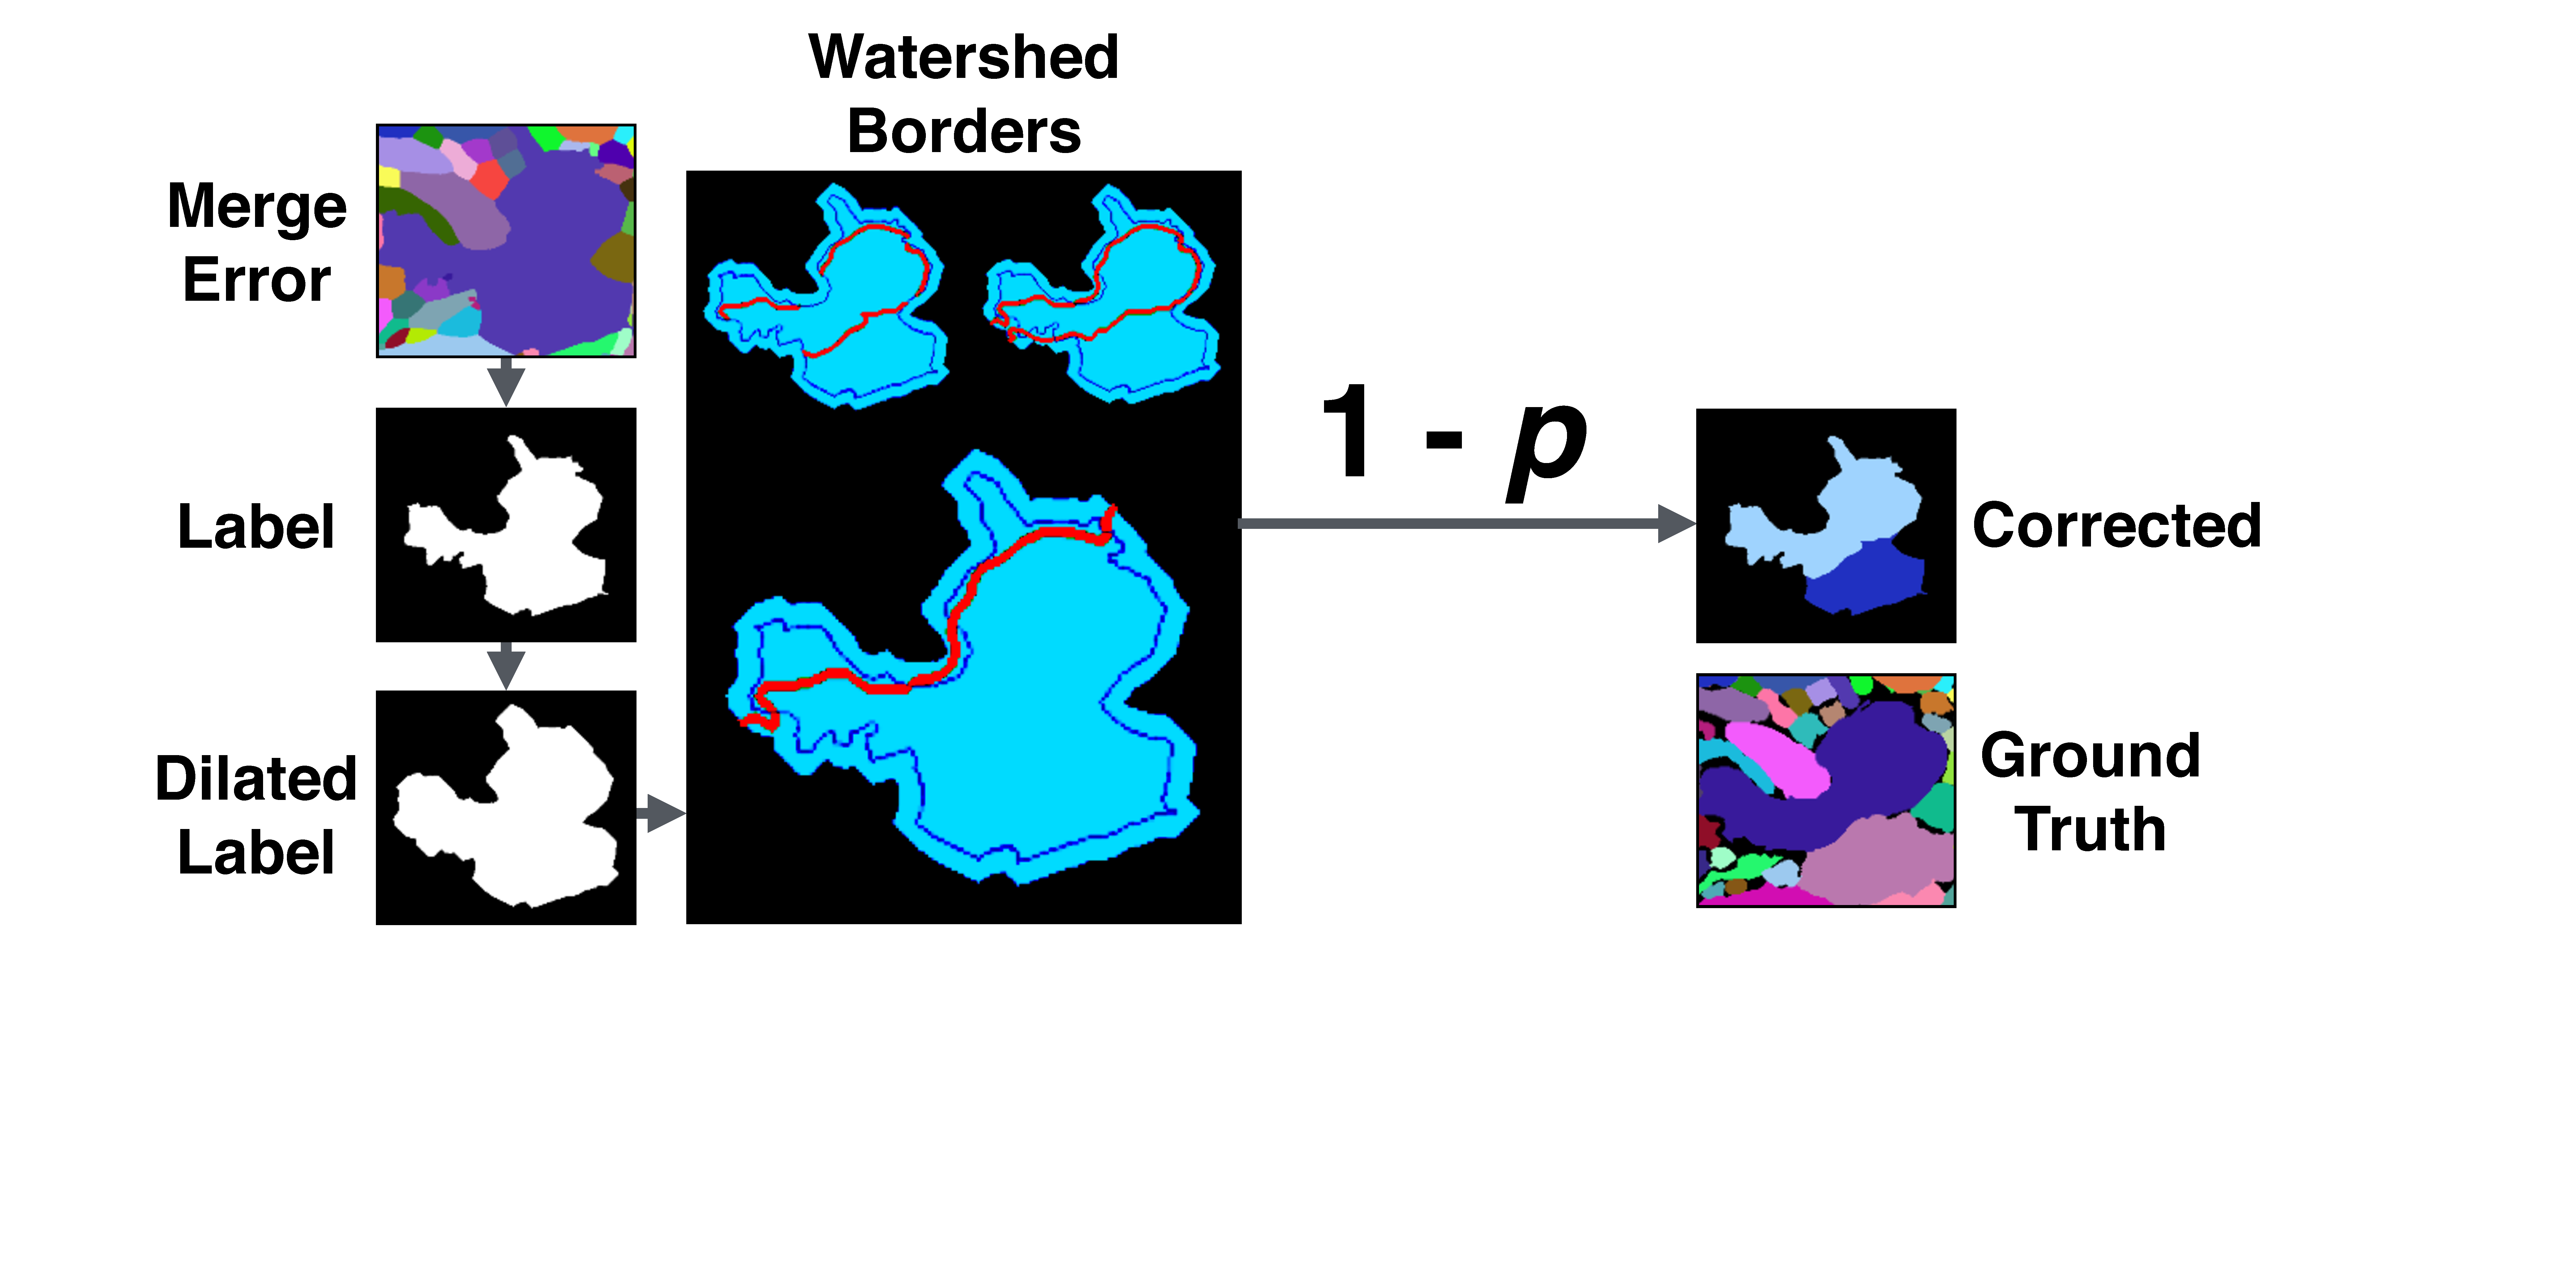
\includegraphics[width=\linewidth]{gfx/merge_error_v4.pdf}
\caption{Updated Figure 4. (not yet)}
\label{fig:merge_error}
\end{figure}


\section{}


{\small
\bibliographystyle{ieee}
\bibliography{egbib}
}

\end{document}
